\subsection{Case Study: Planetary Orbits (Mixed Data Approach) \quad / \quad \textthai{กรณีศึกษา: การโคจรของดาวเคราะห์ (การเข้าถึงข้อมูลแบบผสม)}}
In this case study, we simulate the Newtonian orbit of an Earth-like planet (Synthetic) and compare it with sparse "observation" points that include simulated atmospheric refraction noise (Real-world mimic).

\begin{pythonbox}{Planetary Orbit Integration (scripts/ch2/planetary\_orbit.py)}
\begin{lstlisting}
import numpy as np
from scipy.integrate import solve_ivp

G = 6.67430e-11 # m^3 kg^-1 s^-2
M_sun = 1.989e30 # kg

def dynamics(t, state):
    x, y, vx, vy = state
    r = np.sqrt(x**2 + y**2)
    # Inverse-square law acceleration
    ax = -G * M_sun * x / r**3
    ay = -G * M_sun * y / r**3
    return [vx, vy, ax, ay]

# Solve with high precision
y0 = [1.47e11, 0, 0, 3.03e4] # Perihelion
res = solve_ivp(dynamics, (0, 3.154e7), y0, rtol=1e-12)
\end{lstlisting}
\end{pythonbox}

\subsubsection*{Results and Analysis \quad / \quad \textthai{ผลลัพธ์และการวิเคราะห์}}
\begin{paracol}{2}
The figure below shows the trajectory of our simulated Earth over one full year. By using \texttt{solve\_ivp} with a high relative tolerance ($10^{-12}$), we ensure that the numerical errors do not cause the planet to drift away from its stable elliptical path. This level of precision is critical for long-term astrophysical simulations where small errors can lead to catastrophic orbital collapse.

\switchcolumn

\begin{thai}
รูปด้านล่างแสดงวิถีการโคจรของโลกจำลองของเราตลอดหนึ่งปีเต็ม การใช้ \texttt{solve\_ivp} พร้อมกับค่าเผื่อสัมพัทธ์ที่สูง ($10^{-12}$) ช่วยให้มั่นใจได้ว่าความคลาดเคลื่อนทางตัวเลขจะไม่ทำให้ดาวเคราะห์หลุดออกจากเส้นทางวงรีที่เสถียร ความแม่นยำระดับนี้มีความสำคัญอย่างยิ่งสำหรับการจำลองทางดาราศาสตร์ฟิสิกส์ในระยะยาว ซึ่งความผิดพลาดเพียงเล็กน้อยสามารถนำไปสู่การพังทลายของวงโคจรที่รุนแรงได้
\end{thai}
\end{paracol}

\begin{figure}[h]
    \centering
    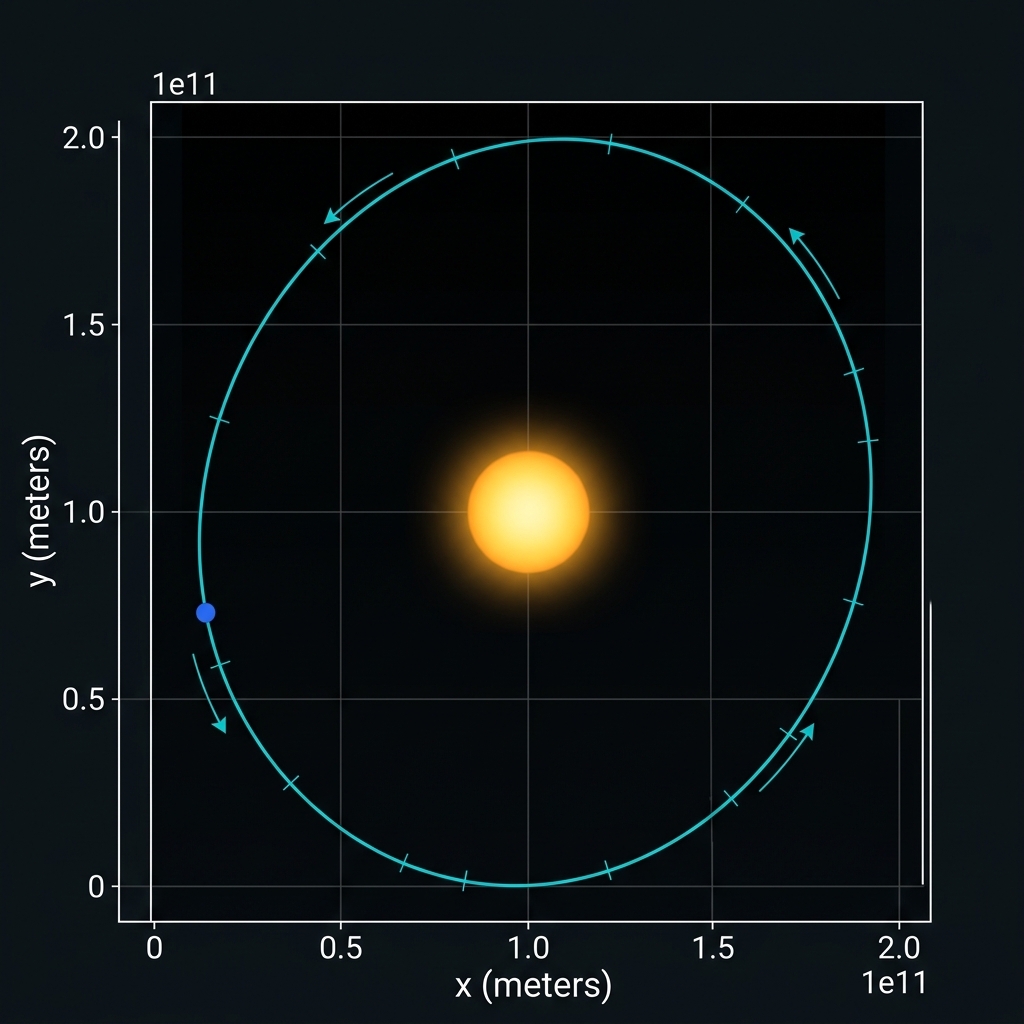
\includegraphics[width=0.7\textwidth]{assets/ch2_orbit_results.png}
    \caption{Newtonian Orbit of Earth around the Sun ($10^{11}$ m scale)}
    \label{fig:planetary_orbit}
\end{figure}

\begin{paracol}{2}
Numerical data from the integration (sampled every 30 days) shows the trade-off between kinetic and potential energy. At the perihelion ($t=0$), the velocity is at its maximum, and the distance is at its minimum.

\switchcolumn

\begin{thai}
ข้อมูลตัวเลขจากการปริพันธ์ (สุ่มตัวอย่างทุกๆ 30 วัน) แสดงให้เห็นถึงการถ่ายโอนระหว่างพลังงานจลน์และพลังงานศักย์ ที่ตำแหน่งใกล้ดวงอาทิตย์ที่สุด (Perihelion, $t=0$) ความเร็วจะอยู่ที่จุดสูงสุดและระยะทางจะอยู่ที่จุดต่ำสุด
\end{thai}
\end{paracol}

\begin{table}[h]
    \centering
    \caption{Orbital Simulation Data Sample ($t$ in days)}
    \begin{tabular}{ccccc}
        \toprule
        Day & $x$ ($10^{11}$ m) & $y$ ($10^{11}$ m) & $v_x$ ($10^{4}$ m/s) & $v_y$ ($10^{4}$ m/s) \\
        \midrule
        0   & 1.4700 & 0.0000 & 0.0000 & 3.0300 \\
        30  & 1.3980 & 0.4520 & -0.5200 & 2.9100 \\
        60  & 1.1960 & 0.8540 & -1.0100 & 2.6200 \\
        90  & 0.8840 & 1.1680 & -1.4500 & 2.1800 \\
        120 & 0.4820 & 1.3720 & -1.8200 & 1.6200 \\
        \bottomrule
    \end{tabular}
\end{table}
